\renewcommand{\thefigure}{\Asbuk{section}.\arabic{figure}}
\renewcommand{\thetable}{\Asbuk{section}.\arabic{table}}
\renewcommand{\thelstlisting}{\Asbuk{section}.\arabic{lstlisting}}

\chapter*{%
  Приложение А \hspace{10cm}
  Точность прогнозирования наблюдений выхода
  линейной стохастической  \hspace{10cm}
  системы второго типа \hspace{12cm}
  (к подразделу~2.3.2)
}
\addcontentsline{toc}{chapter}{%
  Приложение А
  Точность прогнозирования наблюдений выхода \\
  \hspace*{2.8cm} линейной стохастической системы второго типа
}

\setcounter{section}{1}
\setcounter{figure}{0}
\setcounter{table}{0}
\setcounter{lstlisting}{0}

На приведенных ниже рисунках показана зависимость величины~\eqref{eq:dst_linear_predict}
от с.к.о. ошибок наблюдений \( \sigma_{\varepsilon_x}, \sigma_{\varepsilon_y} \) при
различных фактических значениях коэффициента усиления \( \beta \)
линейной стохастической системы второго типа.

\begin{figure}[h]
  \centering
  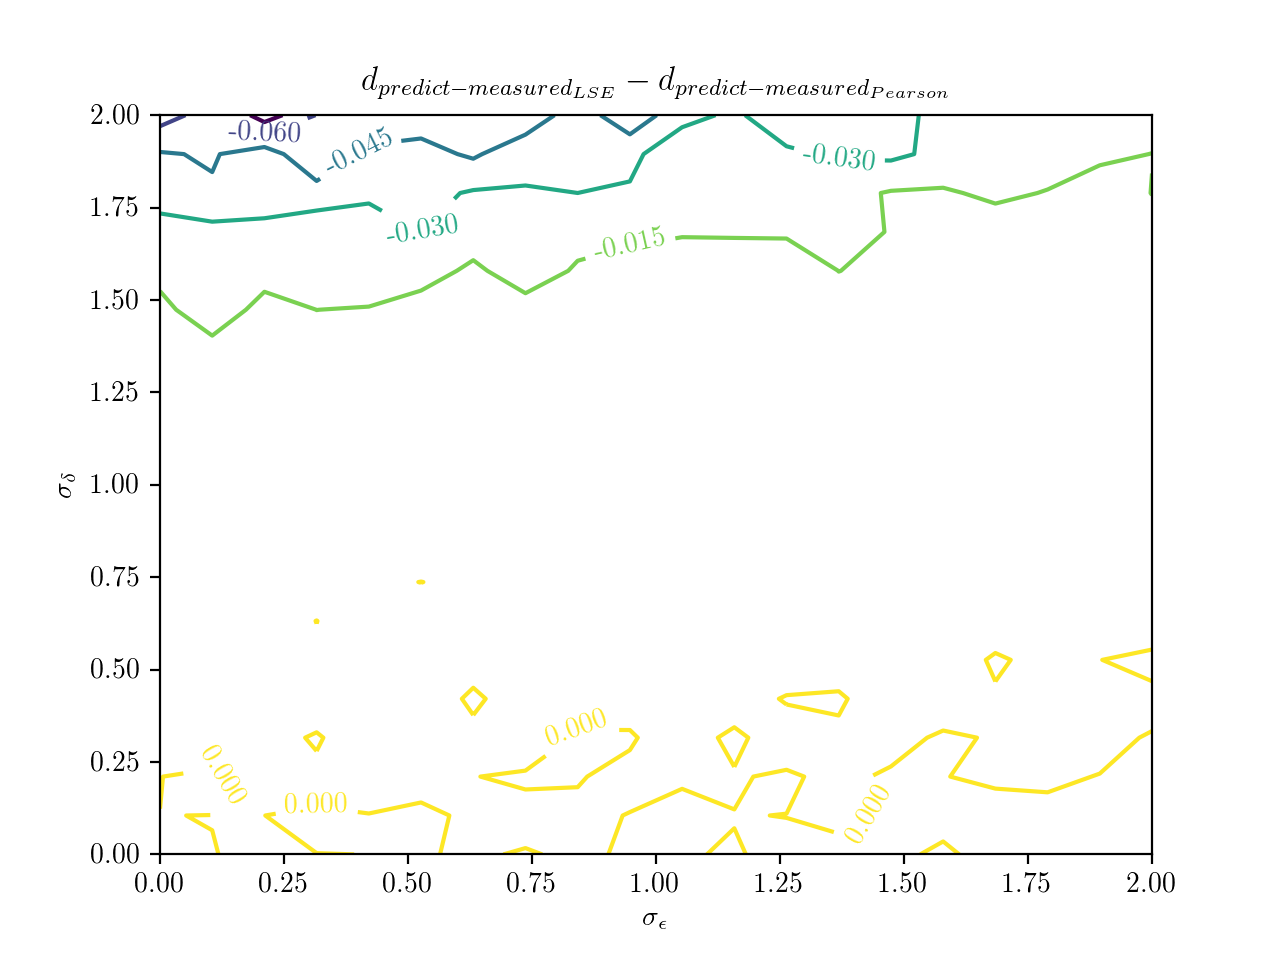
\includegraphics[width=135mm]{fig/linear/predict/beta-0,2_predict-measured.png}
  \caption{Точность прогнозирования наблюдений выхода при \( \beta = 0{,}2 \)}
\end{figure}

\begin{figure}[h]
  \centering
  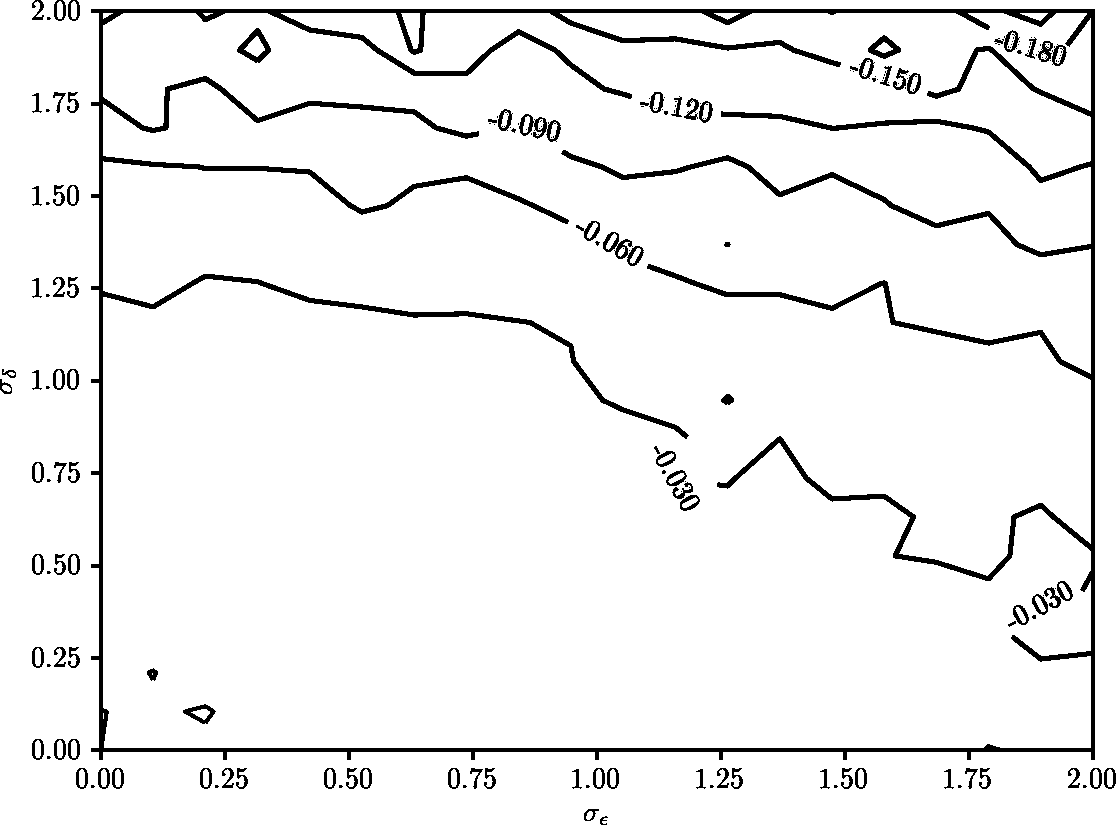
\includegraphics[width=135mm]{fig/linear/predict/beta-1_predict-measured.png}
  \caption{Точность прогнозирования наблюдений выхода при \( \beta = 1\)}
\end{figure}

\begin{figure}[h]
  \centering
  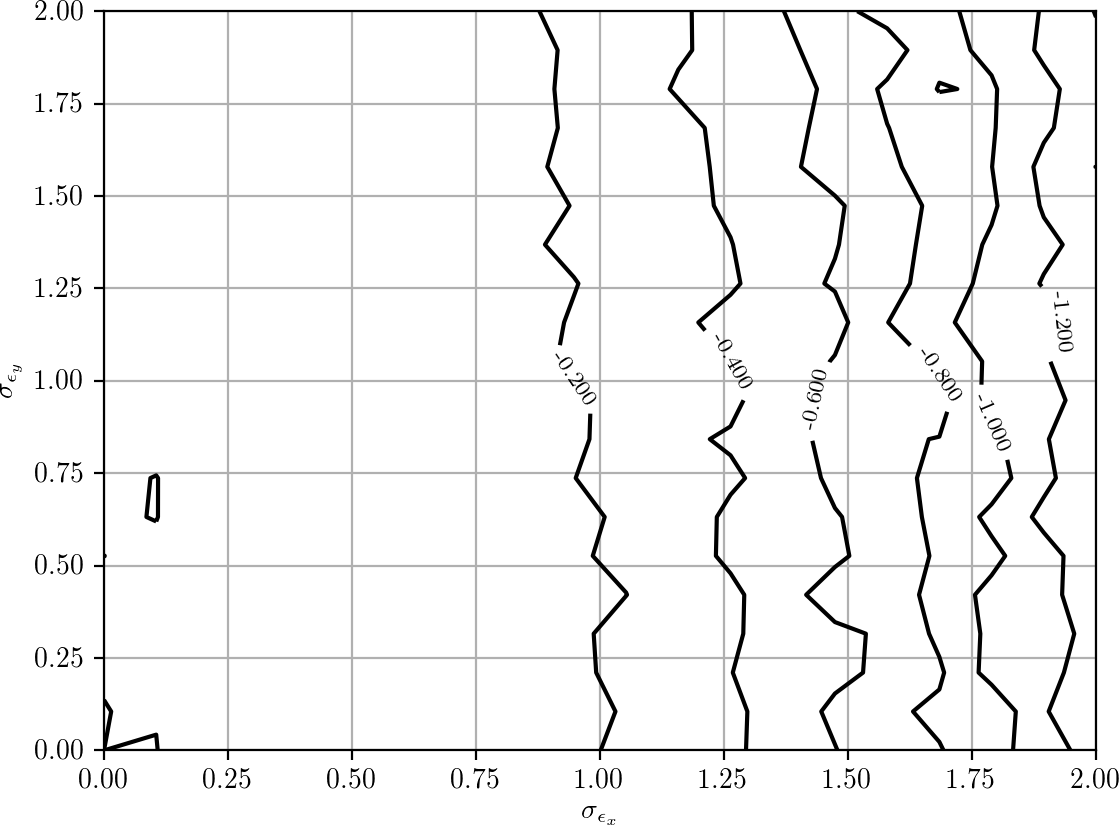
\includegraphics[width=135mm]{fig/linear/predict/beta-5_predict-measured.png}
  \caption{Точность прогнозирования наблюдений выхода при \( \beta = 5 \)}
\end{figure}
